\section{Design}
\label{sec:design}

In this section, the design goals of the proposed approach are discussed.
First, general principles of using LoRa on smartphones are covered.
Second, design goals of a generic LoRa modem firmware are presented.
Third, requirements for a device-to-device chat application are examined.
Finally, thoughts on integrating LoRa into disruption-tolerant networking are presented.

\subsection{Enabling LoRa on Smartphones}
To extend smartphones and other common devices by infrastructure-less communication technologies, a generic interface must be designed.
While these devices offer a variety of communication technologies, only few are shared across different categories of devices.
Ethernet and USB may be available on most devices including laptops and routers, but smartphones can utilize these connections only using special adapters, if at all. 
However, all of the mentioned devices offer Wi-Fi and/or Bluetooth interfaces.
Furthermore, the used approach should be based on low-energy solutions, since in the described scenarios power supply may be limited or not available.
In the following, we present a modem firmware, called \textit{rf95modem},  for LoRa MCUs that can enable access to the LoRa hardware through other communication channels.

\begin{figure}[ht!]
    \centering
    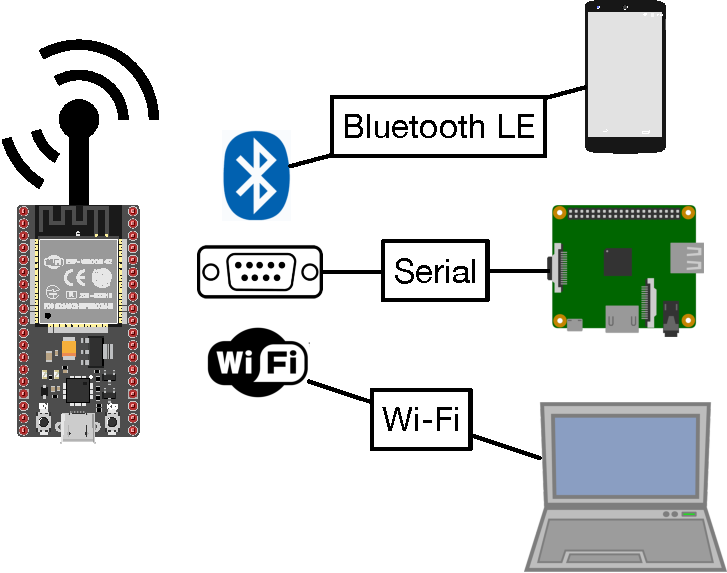
\includegraphics[width=.5\columnwidth]{gfx/rf95modem-connections.pdf}
    \caption{ESP32-based modem board and its connection options for smartphones, single-board computers, and laptops.}
    \label{fig:rf95modem}
\end{figure}

\subsection{Modem Firmware}
Figure~\ref{fig:rf95modem} shows how different devices can be connected to a modem board. 
There are several commercial off-the-shelf micro-controller boards available that include a LoRa transceiver and thus can be used for the proposed functionality.
With our approach, we aim to support the majority of these boards by providing a hardware abstraction layer across all of them.
Thus, the provided implementation supports a wide variety of available boards, e.g., 
the LilyGO TTGO LoRa series\footnote{\url{http://www.lilygo.cn/pro.aspx?FId=t3:50003:3}, Xing Yuan Electronic Technology Co., Ltd., LongGang, Shenzhen, China},
Adafruit's Feather 32u4 and M0 boards \footnote{\url{https://www.adafruit.com/product/3178}, Adafruit Industries, LLC, 150 Varick Street, New York 10013, USA} or 
% the PyCom LoPy4 and FiPy boards\footnote{\url{https://pycom.io/solutions/hardware/}, Pycom, 57 Avenue Road, Cranleigh, Surrey GU6 7LJ, United Kingdom},
the Heltec Automation WiFi LoRa 32 and Wireless Stick (Lite)\footnote{\url{https://heltec.org/proudct_center/lora/lora-node/}, Heltec Automation, Longtan Industrial Park, Chengdu, China}.
Some of these boards only provide LoRa and a serial interface via USB, but others also provide Wi-Fi and Bluetooth.
The modem firmware is supposed to be controllable through AT commands similar to classic modems or various smartphones. 
Thus, no specific device drivers are needed to send and receive data via the \textit{rf95modem} firmware.
Finally, the firmware should be flexible enough and easily configurable to only ship the code actually needed for the device and the scenario in which it is used.


\subsection{A Device-To-Device Messaging Application}
To enable communications in rural areas or in situations after disasters, mobile applications play an outstanding role for various reasons and support a variety of communication technologies like cellular, Wi-Fi, and Bluetooth.
Therefore, we designed a mobile application to support off-grid communication in the scenarios mentioned above.
In particular, in crisis situations, it is important that users do not first have to familiarize themselves with new paradigms or UI/UX concepts and are not confronted with technical terms that are incomprehensible to laypersons.
Therefore, our application should use Bluetooth Low Energy (BLE) as the primary connection technology.
Bluetooth is widely accepted as a technology to create one-to-one connections and exchange data between the involved peers, whereas Wi-Fi is usually used to access information from a central place.
Therefore, the Bluetooth paradigm fits better to the given scenario.
Additionally, Bluetooth is more energy efficient compared to Wi-Fi, which makes it the appropriate technology to use in this case.
To further reduce barriers in app usage, our app should automatically connect to nearby modem devices without any further actions required by the user.
This increases the chances of instant access to the communication infrastructure in cases of emergencies.
The app should also be able to receive messages in the background, e.g., when the user leaves the application.
Additionally, the user should not worry about using a specific mobile device.
It is therefore crucial to provide a platform-independent application that is usable on the most popular mobile platforms iOS and Android.

To get people in contact as fast as possible without prior exchange of IDs, usernames or alike, the application should follow a public message board paradigm, similar to Twitter, where users can post short messages to a publicly visible channel.
Here, users can send messages visible for all and ask for help or provide status information.
This approach gives users easy and fast access to a communications method.
Users should have an easy and fast way to find new channels and create channels for specific topics.
Finally, users should be presented with a common and familiar look-and-feel including accessibility features so that no one is excluded.

\subsection{Disruption-tolerant Networking}
For crisis scenarios, DTN is a technology to enable infrastructureless communication using an emergency infrastructure in conjunction with existing devices of users (\cite{baumgartner2016experimental,lieser2017architecture}). 
DTNs benefit from a large number of devices storing and forwarding messages to other devices when they become available. 
Today, end user focused DTNs are mostly based on ad-hoc Wi-Fi and Bluetooth, since these are available in the mobile devices used by the users. 
Due to slow data rates and duty cycle restrictions introduced by regulation, LoRa in DTNs is not suited for larger data transmissions, such as multimedia content, but is helpful to transmit context information or small messages.
LoRa can be used to connect different local clouds of people, where smaller messages available inside the cloud can be transmitted to another cloud. 
Modern DTN routing algorithms use context information to reduce overheads introduced by unnecessary transmission~(\cite{graubner2018opportunistic}). 
We propose to add LoRa to existing delay- and disruption-tolerant networks to enable larger spatial low-bandwidth coverage, in order to propagate small messages and context information. 
To facilitate the use of LoRa in DTN networks, an exemplary integration should be implemented that can use LoRa via Bluetooth, Wi-Fi, or a serial connection and thus is available on mobile devices and static nodes added in crisis scenarios.
